\documentclass{scrartcl}

\usepackage{amssymb}
\usepackage{amsmath}
\usepackage{tikz}

%from Kuan, C.-M. (2008). ``Artificial neural networks,'' in Durlauf, S. \& Blume, L. (Eds.). (2008). \textit{The New Palgrave Dictionary of Economics}, 2nd Ed. London: Palgrave Macmillan.

\begin{document}

	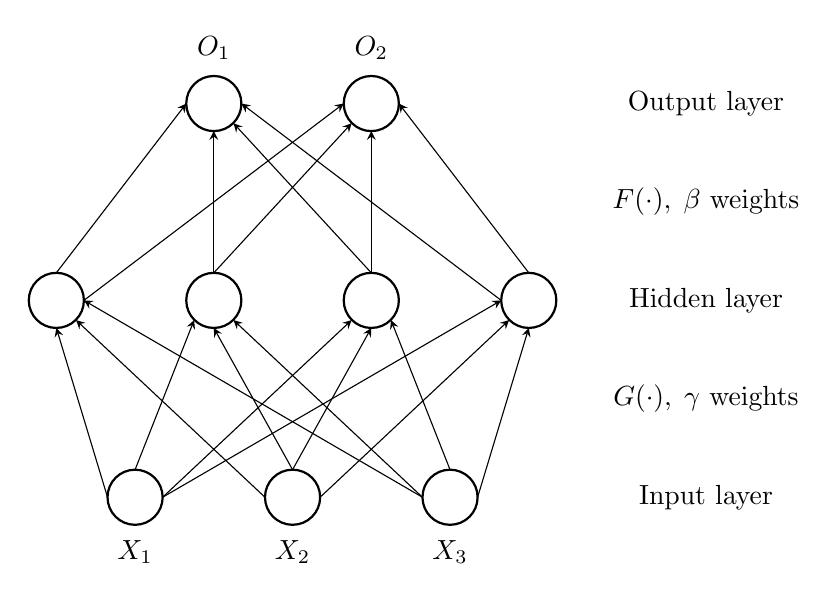
\begin{tikzpicture}[>=stealth]
	\foreach \z in {1,3}
	\filldraw[fill=white,thick] (\z,5) circle (0.35);
	
	\foreach \y in {-1,1,3,5}
	\filldraw[fill=white,thick] (\y,2.5) circle (0.35);
	
	\foreach \x in {0,2,4}
	\filldraw[fill=white,thick] (\x,0) circle (0.35);

	%Hidden--Output	
	\draw[->] (-0.65,2.5)--(2.65,5);	%left circle
	\draw[->] (-1,2.85)--(0.65,5);
	%
	\draw[->] (1,2.85)--(1,4.65);
	\draw[->] (1,2.85)--(2.75,4.75);
	%
	\draw[->] (3,2.85)--(1.25,4.75);
	\draw[->] (3,2.85)--(3,4.65);
	%
	\draw[->] (4.65,2.5)--(1.35,5);		%right circle
	\draw[->] (5,2.85)--(3.35,5);
	
	%Input--Hidden
	\draw[->] (-0.35,0)--(-1,2.15);
	\draw[->] (0,0.35)--(0.75,2.25);
	\draw[->] (0.35,0)--(2.75,2.25);
	\draw[->] (0.35,0)--(4.65,2.5);
	%
	\draw[->] (1.65,0)--(-0.75,2.25);
	\draw[->] (2,0.35)--(1,2.15);
	\draw[->] (2,0.35)--(3,2.15);
	\draw[->] (2.35,0)--(4.75,2.25);
	%
	\draw[->] (3.65,0)--(-0.65,2.5);
	\draw[->] (3.65,0)--(1.25,2.25);
	\draw[->] (4,0.35)--(3.25,2.25);
	\draw[->] (4.35,0)--(5,2.15);
	
	%labels
	\node at (1,5.7) {$O_1$};
	\node at (3,5.7) {$O_2$};
	\node at (0,-.7) {$X_1$};
	\node at (2,-.7) {$X_2$};
	\node at (4,-.7) {$X_3$};
	%
	\node at (7.25,5)	{Output layer};
	\node at (7.25,3.75){$F(\cdot),\;\beta$ weights};
	\node at (7.25,2.5)	{Hidden layer};
	\node at (7.25,1.25){$G(\cdot),\;\gamma$ weights};
	\node at (7.25,0)	{Input layer};
	\end{tikzpicture}
	
	\vspace{0.75cm}
	
	\hspace{0.8cm}
	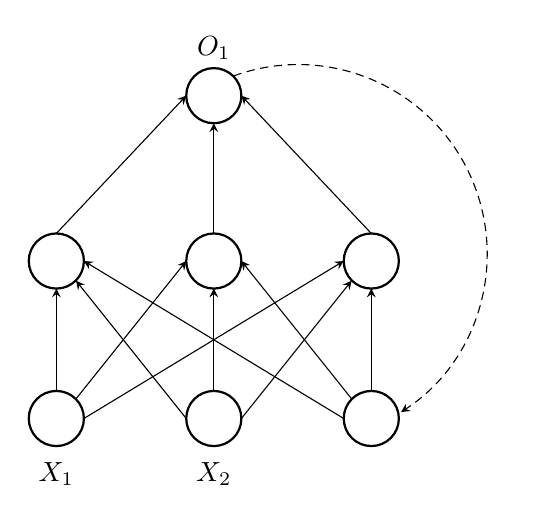
\begin{tikzpicture}[>=stealth]
	\filldraw[fill=white,thick] (0,4.1) circle (0.35);
	\foreach \x in {-2,0,2}
	\filldraw[fill=white,thick] (\x,2) circle (0.35);
	\foreach \y in {-2,0,2}\
	\filldraw[fill=white,thick] (\y,0) circle (0.35);
	
	%Hidden--Output
	\draw[->] (-2,2.35)--(-0.35,4.1);
	\draw[->] (0,2.35)--(0,3.75);
	\draw[->] (2,2.35)--(0.35,4.1);
	
	%Input--Hidden
	\draw[->] (-2,0.35)--(-2,1.65);
	\draw[->] (-1.75,0.25)--(-0.35,2);
	\draw[->] (-1.65,0)--(1.65,2);
	%
	\draw[->] (-0.35,0)--(-1.75,1.75);
	\draw[->] (0,0.35)--(0,1.65);
	\draw[->] (0.35,0)--(1.75,1.75);
	%
	\draw[->] (1.65,0)--(-1.65,2);
	\draw[->] (1.75,0.25)--(0.35,2);
	\draw[->] (2,0.35)--(2,1.65);
	
	%labels
	\node at (0,4.7) {$O_1$};
	\node at (-2,-.7) {$X_1$};
	\node at (0,-0.7) {$X_2$};
	
	%recurrent arrow
	\draw[->,densely dashed] (0.25,4.35) arc (110:-57:2.4cm);
	\end{tikzpicture}
	%this is a Jordan recurrent network b/c back-arrow goes from output to input
	
	\vspace{0.75cm}
	
	\hspace{-1.82cm}
	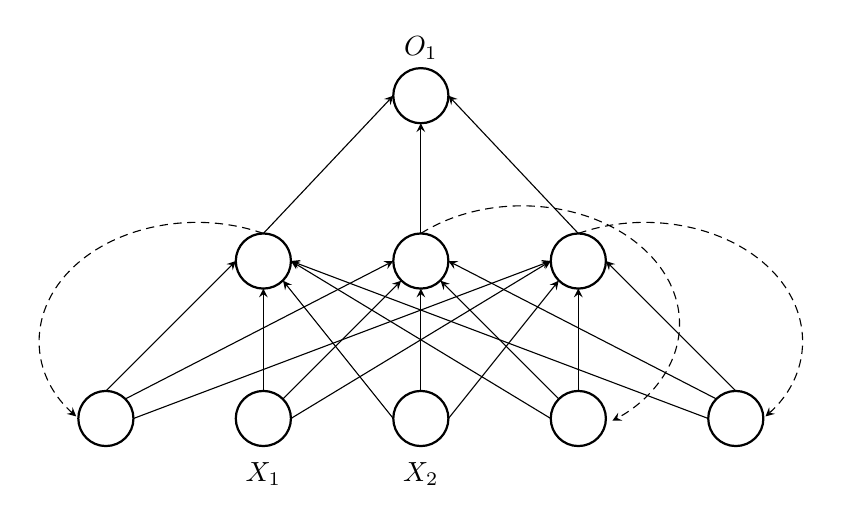
\begin{tikzpicture}[>=stealth]
	\filldraw[fill=white,thick] (0,4.1) circle (0.35);
	\foreach \x in {-2,0,2}
	\filldraw[fill=white,thick] (\x,2) circle (0.35);
	\foreach \y in {-4,-2,0,2,4}\
	\filldraw[fill=white,thick] (\y,0) circle (0.35);
	
	%Hidden--Output
	\draw[->] (-2,2.35)--(-0.35,4.1);
	\draw[->] (0,2.35)--(0,3.75);
	\draw[->] (2,2.35)--(0.35,4.1);
	
	%Input--Hidden
	\draw[->] (-2,0.35)--(-2,1.65);
	\draw[->] (-1.75,0.25)--(-0.25,1.75);	%NB: diff from Jordan
	\draw[->] (-1.65,0)--(1.65,2);
	%
	\draw[->] (-0.35,0)--(-1.75,1.75);
	\draw[->] (0,0.35)--(0,1.65);
	\draw[->] (0.35,0)--(1.75,1.75);
	%
	\draw[->] (1.65,0)--(-1.65,2);
	\draw[->] (1.75,0.25)--(0.25,1.75);		%NB: diff from Jordan
	\draw[->] (2,0.35)--(2,1.65);
	
	%Hidden--Input
	\draw[->] (-4,0.35)--(-2.35,2);
	\draw[->] (-3.65,0)--(1.65,2);
	\draw[->] (-3.75,0.25)--(-0.35,2);
	%
	\draw[->] (3.75,0.25)--(0.35,2);
	\draw[->] (3.65,0)--(-1.65,2);
	\draw[->] (4,0.35)--(2.35,2);
	
	%labels
	\node at (0,4.7) {$O_1$};
	\node at (-2,-.7) {$X_1$};
	\node at (0,-0.7) {$X_2$};
	
	%recurrent arrows
	\draw[->,densely dashed] (-2,2.35) arc (65:220:2cm and 1.5cm);
	%\draw[->,densely dashed] (0,2.35) arc (50:235:2cm and 1.5cm);		%55 & 230 works too
	\draw[->,densely dashed] (0,2.35) arc (130:-55:2cm and 1.5cm);		%125 & 50 works too
	\draw[->,densely dashed] (2,2.35) arc (115:-40:2cm and 1.5cm);
	\end{tikzpicture}
	%this is a Elman recurrent network b/c back-arrows go from hidden to input
	
\end{document}